% Preamble
% Global
\documentclass[
    parskip=full,
    a4paper
]{scrartcl}
\usepackage{blindtext}
\usepackage[utf8]{inputenc}
\usepackage{etoolbox}

\usepackage{hyperref}
\hypersetup{
    colorlinks,
    citecolor=black,
    filecolor=black,
    linkcolor=black,
    urlcolor=black
}

% Graphics
\usepackage{pdfpages}
\usepackage{graphicx}
\usepackage{xcolor}
\usepackage[many]{tcolorbox}
\usepackage{etoolbox}

% Diagrams
\usepackage{tikz-er2}
\usetikzlibrary{positioning}
\usetikzlibrary{shadows}

\tikzstyle{every entity} = [top color=white, bottom color=blue!30,
draw=blue!50!black!100, drop shadow]
\tikzstyle{every weak entity} = [drop shadow={shadow xshift=.7ex,
        shadow yshift=-.7ex}]
\tikzstyle{every attribute} = [top color=white, bottom color=yellow!20,
draw=yellow, node distance=1cm, drop shadow]
\tikzstyle{every relationship} = [top color=white, bottom color=red!20,
draw=red!50!black!100, drop shadow]
\tikzstyle{every isa} = [top color=white, bottom color=green!20,
draw=green!50!black!100, drop shadow]

% Lists
\usepackage{enumitem}
\setlist{nosep} % or \setlist{noitemsep} to leave space around whole list

% Layout
\usepackage[margin=1in]{geometry}
\usepackage{setspace}
\usepackage[utf8]{inputenc}
\usepackage[english]{babel}
\setstretch{1.3}
% \setlength{\parindent}{0em}
% \setlength{\parskip}{1em}

% Inline-code
\usepackage[outputdir=./_build]{minted}
\definecolor{dhscodebg}{rgb}{0.01,0.199,0.1}
\setminted{
    breaksymbolleft=,
    fontsize=\scriptsize,
    baselinestretch=1.1,
    % bgcolor=dhscodebg,
    % rulecolor=\color{gray!40},
    % framesep=\fboxsep,
    % frame=single,
    % framesep=10pt
    % framerule=2pt,
    xleftmargin=2.5em,
    linenos,
    breaklines,
    tabsize=4
}
\usemintedstyle{tango}
\BeforeBeginEnvironment{minted}
{\begin{tcolorbox}[
            breakable,
            boxrule=0.2pt,
            colback=gray!40,
            % toprule=1pt,
            % rule=1pt,
            arc=0pt
        ]}\AfterEndEnvironment{minted}{\end{tcolorbox}}

% Bibliography
\usepackage{natbib}
\usepackage{bibentry}
\nobibliography*

% Title
\title{Unintended effects of UCT's academic striking; an exploration of new software metaphors for the information age.}
\author{Zach Smith}
\date{\today}

% Document
\begin{document}

% Title page
\maketitle
\newpage

%  TOC
\tableofcontents
\newpage

% Content
\section{Introduction}
Despite major disruptions to the University of Cape Town's teaching curriculum in 2016 xxx, the academic year was completed successfully with only minimal disruptions to the calendar schedule. Despite xxx hours of teaching time lost, xxx days of closing the university, course curriculum remained constant and exams tested a similar amount of material as had been previously tested.

One of the reasons the university could absorb such disruptions is due to their implementation of learning management software - their 'Vula' system, which is based on the 'Sukai' platform.

The trend of educational institutions has been to increasingly implement and rely on such software and UCT is no exception. Looking at a graph showing the uptake of such systems throughout globally acclaimed educational institutes shows just how important they have become xxx. A plethora of competing educational tools exist; Blackboard, Canvas, Sukai to name a few, all with a fairly comparable feature list xxx.

A key feature is ability to host and deliver course content via an online platform, taking advantage of functionality that such a platform can provide - in this case with reference to tracking of platform and content usage. With reference specifically to the Sakai platform, it is possible to follow which students accessed which resources and the timing of such events.

The striking at the University of Cape Town provides a unique opportunity to analyze this data as a comparison between classroom learning augmented by online tools vs primary reliance on online tools over an extended period by the same learners. Effectively a blind-control was inadvertently created that allows assessment of a single group of students in two isolated environments in terms of their resultant grades.

\section{Tech approach}
As adopted all over the working world, Microsoft Excel (and other spreadsheet tools) have made using computing power available to all the general population such that global economies have been able to proliferate as quickly as they have. xxx

But we are fast reaching the limits of what Excel-based computing is able to achieve for two reasons:

\begin{enumerate}
    \item Local memory will not accommodate the increasing amount of data available
    \item Moor's law will eventually create a hard limit on the amount of data that a personal machine can process.
\end{enumerate}

As such, a new user technology stack needs to be thought out that allows user's easier access to more computing power. It is the opinion of this author that such a tech-stack will no-longer be the over-opinionated GUIs as current spreadsheets represent, but a regression back to text-based terminals that allow for more configurable and bespoke computer usage. With increasingly easy-to-learn programming APIs and increasingly complicated GUIs, and according to xxx, it is no longer more difficult to learn a high-level programming language like JavaScript/Python/Ruby/etc than it is to learn a GUI. Configuration is also easier than it has been with the emergence of YAML, JSON, etc. over XML. And programming directly allows for far more configuration than a GUI can ever provide.

This is not to say that the prevalence of GUIs will diminish over time, but rather that their usage will shift to facilitate easier implementation of high-level programming languages.

It will definitely require a shift in mentality, however, to move away from Microsoft-provided metaphors that have become so ubiquitous that most users don't even use that they are using metaphors at all. Users think of MS Word 'documents' and their 'pages' as if they were just as real as the tangible items that they are based on.

Part of this project will involve a breakdown of common visual metaphors used in every-day data analysis / processing and discuss how those metaphors could evolve to accommodate similar processes as currently in use but with the ability to process exponentially greater amounts of data.
% \bibliography{../../bibliography/msc_citations}

\section{Student Data}
Events file has 44420509 lines.

\section{Calculation with CouchDB}
As a means of testing feasibility of building indexes across large amounts of documents in CouchDB, I installed the database locally on a Windows 10 personal PC. It took a little over an hour to parse 44 million CSV rows into the database, with nETL using a maximum of around 450MB of system memory and negligible CPU/Disk capacity.

There is no way of calculating indexing times of CouchDB views, so I created a simple index for benchmark purposes:

\begin{minted}{javascript}
function(doc){
    if (doc.type_) {
        emit(doc.type_, 1);
    };
};
\end{minted}

And found that it took a little over 3 hours to build the index on my machine. The view as written above will have to 'touch' every document in the database, allowing a comparative qualitative estimate for the amount of time other indexes will be built. In other words, since an index is already touching every document in the database, the time complexity is O(n) in terms of the document scan and this would hold true regardless of the logic of the index creation itself. So indexes that process a similar number of documents would take a similar amount of time to be created with:

\begin{enumerate}
    \item An allowance for how long it would take to do a linear scan of each document for the 'type\_' property (so documents with more properties would increase index-build time)
    \item An allowance for how many steps the 'emit' function call requires; each of which would require linear scans of document objects and other calculations. i.e. longer documents == longer index-build times.
\end{enumerate}

In terms of the actual indexing itself, CouchDB includes in its installation a query engine identified by 'couchjs.exe'. The actual MapReduce implementation within CouchDB is strictly tied to the Erlang core and could not be altered without major changes to the source code. Opinionated implementation of MapReduce within the CouchDB database stack, makes it's use-case limited compared to other systems that have become synonymous with the 'big-data' stack - including Hadoop, Google xxx, Microsoft xxx, Amazon xxx stacks.

CouchDB's MapReduce pipeline works something along the lines of

\begin{verbatim}
Map Functions executed in parallel, with [key, value] output collected by CouchDB's main Erlang process
=> Grouping
=> Reduce (+/- Rereduce)
\end{verbatim}

The limitations of this pipeline are:

\begin{enumerate}
    \item You can only run the pipeline once. Additional grouping after a reduction is not possible
    \item Handling the rereduce argument makes writing custom reduce functions challenging
\end{enumerate}

For the two reasons mentioned above, although MapReduce CAN be used to implement SQL-like joins, CouchDB's implementation can't be. Instead it is necessary to utilize a 3rd party function to convert grouped [key, value, value, value, value, etc] output from MapFunctions (with group=true) into 'joined' documents. This is easily achievable via two mechanisms:

\begin{enumerate}
    \item Using CouchDB 'list' functions
    \item Using a 3rd party tool external to the CouchDB application itself
\end{enumerate}

todo: mentions couch lists enumerator functionality


\section{Sakai Event data}

\begin{figure}[h]
    \centering
    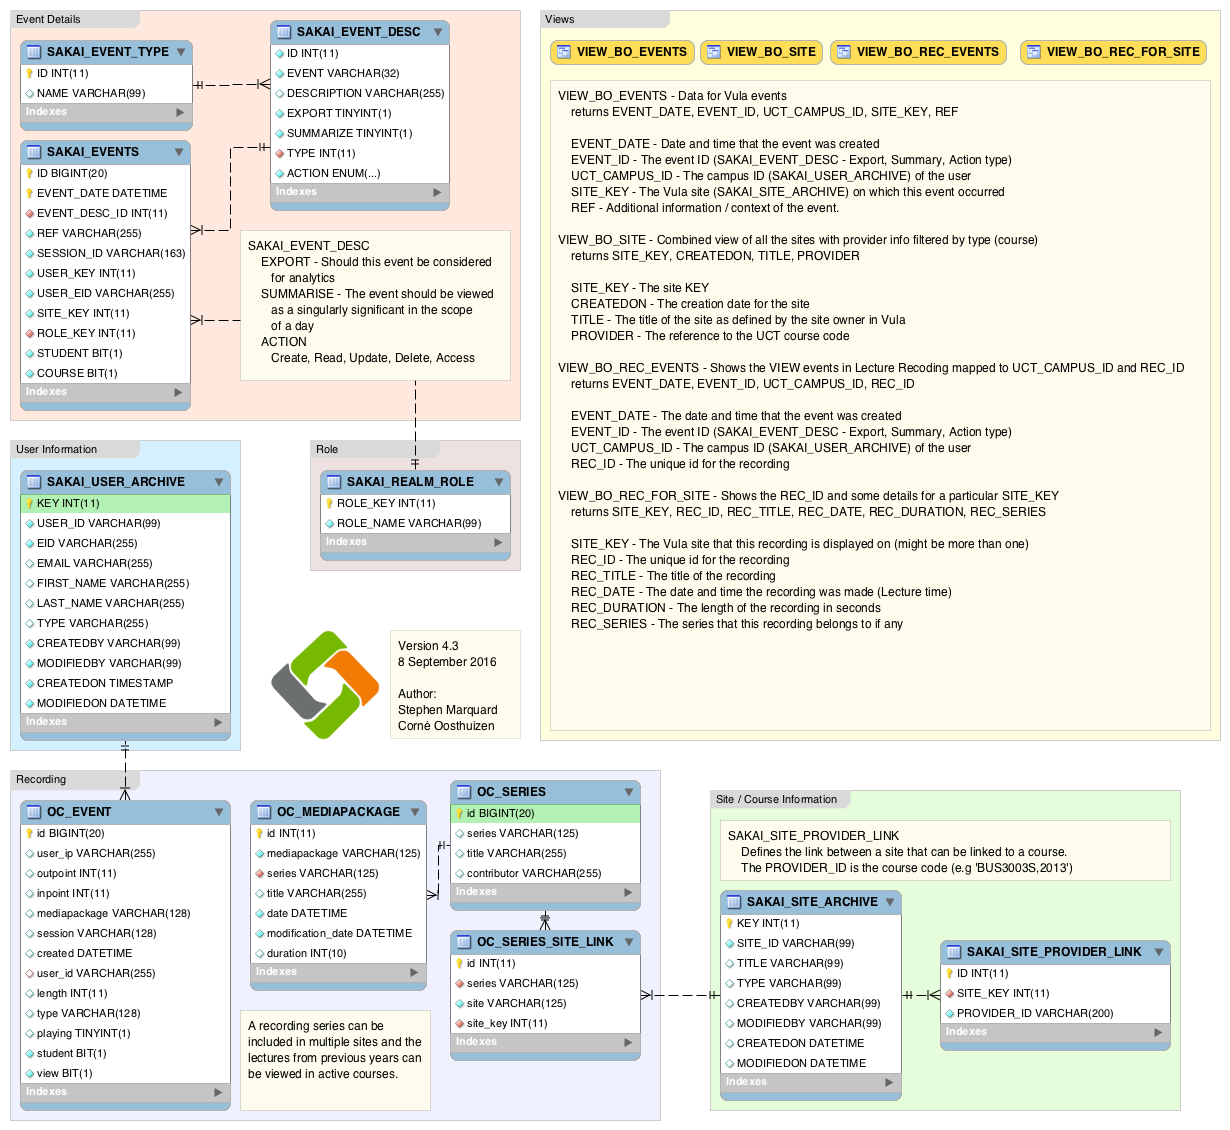
\includegraphics[scale=0.4]{./resources/figures/sakaiEventModel}
    \caption[Sakai]{Model of Sakai browser events as modeled in the RDBMS}
    \label{Sakai}
\end{figure}

Sakai is open source software, meaning that it is fairly straightforward finding information on how it's data-layer is modeled. In this case, browser events are registered as xxx. The University of Cape Town processes the raw event data to model events as represented in \ref{Sakai}. This greatly cuts down on the amount of data that a user needs to process and summarizes all a user's browser interaction on the Sakai site as 'types' of events. These include just 6 categories:

\begin{table}[]
    \centering
    \begin{tabular}{|l|l|}
        \hline
        Event ID & Event Description \\ \hline
        1        & Administration    \\
        2        & Assessment        \\
        3        & Communication     \\
        4        & Content           \\
        5        & Presence          \\
        6        & System            \\ \hline
    \end{tabular}
    \caption[Sakai Event Types]{All user interaction on the Sakai browser frontend can be categorized as a part of one of these events}
    \label{SakaiEventTypes}
\end{table}

For the purposes of this project, only events of type 'presence' will be considered. These are thought to be representative of a students usage of Sakai on the basis that, in most cases, a student would login to the platform with the intention of transacting in a 'learning' sense.

Retrieving events of type 'presence', a natural join (i.e. a join across common columns) is required. Such a join; \textit{R(a,b)} joined with \textit{S(b,c)} joined with \textit{T(c,d)} (where \textit{R}, \textit{S} and \textit{T} are relations and \textit{a}, \textit{b}, \textit{c}, \textit{d} are attributes) could be expressed via the following SQL (SQL Server syntax):

\begin{minted}{sql}
SELECT
[R].[a],
[T].[d]
FROM [R]
LEFT JOIN [S] on [S].[b] = [R].[b]
LEFT JOIN [T] ON [T].[c] = [S].[c]
\end{minted}

As mentioned by \cite{mining2011}, within a MapReduce context such a join can be achieved via:
\begin{enumerate}
    \item A Map function: iterating through all tuples \textit{(commonField, fieldList)} of all relations and producing a key-value pair of the form \textit{(commonField, (Relation, fieldList))}
    \item An implicit group function: group all Map output as a list of tuples per common key of the form \textit{(id, ((R,A), (S, C), (T,D), etc))}
    \item A Reduce function to produce the desirable attributes across the joined tuples \textit{(A,D)} where attribute \textit{C} is of a particular value
\end{enumerate}

As discussed above, a multi-way join is impossible within CouchDB's implementation of MapReduce. As mentioned by \cite{chandar2010} and others xxx multi-way joins need multiple map phases, which is not a possibility using the CouchDB software. CouchDB's implementation of MapReduce is opinionated in that it expects xxx and xxx and doesn't allow for xxx.

TODO: Ask about multiway joins on the Slack channel.

CouchDB's MapReduce implementation allows for a single Map - Group - Reduce pipeline, which is limiting in comparison to frameworks such as xxx, xxx, etc. This means that CouchDB's ability to join is limited by what the common keys of the entities are; only a single 'common' key is allowed since to join in Couch's MapReduce that key needs to be emitted for every document included in the join.

The query above needs to run the join of \textit{R(a,b)} with \textit{S(b,c)} prior to joining the result with \textit{T(c,d)} since a common property - \textit{c} needs to be created for the relation \textit{R} before tuples for \textit{R} and \textit{T} can be grouped by a common key (\textit{c}).


\subsection{Data Analysis}
s
% \bibliography{../../bibliography/msc_citations}

\section{MapReduce}
This should be a general overview of how Map Reduce actually works and why it was worth thinking about.

\subsection{What is MapReduce?}
As discussed by \cite{mining2011}, data-centered applications that make use of a large amounts of data have spurred the development of distributed computing using commodity hardware instead of super-computers. <xxx google big table, amazon hive>. Distributed file systems have subsequently been developed as a response to computing on dispersed clusters of commodity hardware that enables, amongst other things, distributed data-processing. \cite{mining2011} refers to the combination of clustered commodity hardware, a distributed file system, and the wide variety of software aimed to be executed on this new platform as the 'New Software Stack'.

Intrinsic to this 'New Software Stack' is the idea of MapReduce \cite{mining2011}; a logical framework for approaching data analysis in a distributed way. With initial implementations of MapReduce aimed at lower level data handling within the file system, it has become clear that it is useful across the entirety of software abstraction levels; including implementations of the SQL specification, the extent of which this is possible being dependent on specific MapReduce implementations. \cite{mining2011} show a variety of different ways that data can be queried in a SQLesque way.

MapReduce is actually quite an old idea <xxx> that first rose to prominence as the framework implemented to rank web pages implemented by Google, graph analysis and other such clean data sources <xxx>. But in fact, MapReduce may be just as useful as a means of 'normalizing' irregular data within a standard relational context (the subject of this project) due to the versatility of the different components within the MapReduce specification.


\subsection{Data manipulation with MapReduce}
This section should compare standard SQL operations to how they are implemented in MapReduce, with the conclusion that everything is possible that a standard SQL database does, via MapReduce

- Discuss how the book shows it is possible to implement different families of algorithms using MapReduce
- Name a couple of them, and then contrast MapReduce algorithm analysis in terms of time and space complexity
- communication cost model
- complexity theory

The point of me choosing to use MapReduce is that the Map functions are split across many of nodes. And that this makes it easy to calculate dispersedly. So I should get some citations of why this is more difficult and more expensive than doing the same on a relational database. Perhaps this could be as simple as having to maintain a file system that is dispersed across multiple physical computing devices - requiring special hardware.
\section{CouchDB}

\subsection{MapReduce overview}
TODO: This should be a summary of how MapReduce can indeed be used to implement the entire specification of SQL. Basically this is a summary of the book by the Google guys

\subsection{Cluster Setup}
Similarly to the ubiquity of Microsoft Office metaphors to the point that it is easy to forget that they are metaphors at all, it is easy to forget that the personal computer is in itself a metaphor for working with a processing chip. While it is possible to install CouchDB on a Windows personal computer, there is very little incentive to do so since you would effectively nullify the benefits of working with a dispersed, JSON-based, HTTP-fronted database.

CouchDB is a new animal on the database market, with development started by xxx in xxx primarily as a tool to xxx. The current release, CouchDB 2.1 has a variety of features that may finally make it feasible to replace the way technology has traditionally been used in workplace roles. A summary of CouchDB's key features is:

\begin{enumerate}
    \item Semi-structured data storage allows for easier use by people without prior database experience
    \item An HTTP interface effectively brings database communication out of the stone age and makes interacting with a database on a low level accessible to anyone who can code a line of JavaScript
    \item A MapReduce-based query engine allows for easily creating indexes that can be calculated via distributed computing
    \item And very easy/cheap cluster setup when compared to traditional DBMSs
\end{enumerate}

With these benefits in mind, this project explores the usage of CouchDB as a persistent (but temporary) dispersed data-processing engine for student data in the form of:

\begin{enumerate}
    \item A tool for easily configuring CouchDB clusters with enough nodes to handle the required data volume
    \item An approach for easily designing CouchDB MapReduce indexes, implementing them and running them
\end{enumerate}

CouchDB is open-source software with free binary distributions for a Windows, Max, and Linux environment. With the intent of clustering many server instances, each with it's own instance of the CouchDB software, only Linux is feasible since it is released as free software (GPL license). Combined with affordable, virtual, managed servers such as those offered by Digital Ocean, AWS, Hetzer, Linode to name a few (including several South Africa-based companies), clustered computing is very much within the reach of everyday consumers. Setting up several Ubuntu Xenial/CouchDB 2.1 instances is no more complicated than running a few commands on a Linux terminal. While there is still some technical understanding required in terms of security, it would be fairly straightforward to package 'setup' scripts for non-technical users giving users the potential to utilize CouchDB clusters in their own right.

For the purposes of this MSc, several instances of Hetzner's CX20 virtual cloud servers were used. xxx

A complete list of the commands required for a basic installation of an Ubuntu Xenial server supporting a CouchDB 2.1 installation is as follows:

\begin{minted}{sh}
# Set hostname of server
hostname <hostname>; rm /etc/hostname; touch /etc/hostname; echo <hostname> >> /etc/hostname; chmod 466 /etc/hostname;

## Install basic tooling 
# GCC collection (GNU make and GNU compiler tools)
apt-get update
apt-get install build-essential -y

# Update openssl to 1.0.2l
cd /usr/src
wget https://www.openssl.org/source/openssl-1.0.2l.tar.gz
tar -zxf openssl-1.0.2l.tar.gz
cd openssl-1.0.2l
./config
make
make test
make install
mv /usr/bin/openssl /root/
ln -s /usr/local/ssl/bin/openssl /usr/bin/openssl

# Python
apt-get update
apt-get install python -y

# libcurl
apt-get update
apt-get install libcurl4-openssl-dev -y

# ICU
apt-get update
apt-get install libicu-dev -y

# (Optional - this enables automated installations) preseed debconf to answer CouchDB installation wizard automatically
debconf-set-selections <<< 'couchdb couchdb/bindaddress string 0.0.0.0'
debconf-set-selections <<< 'couchdb couchdb/cookie string monster'
debconf-set-selections <<< 'couchdb couchdb/mode string clustered'
debconf-set-selections <<< 'couchdb couchdb/nodename string couchdb@<hostname>'
debconf-set-selections <<< 'couchdb couchdb/adminpass password <password>'
debconf-set-selections <<< 'couchdb couchdb/adminpass_again password <password>'

# register CouchDB package with the server package manager and install
echo 'deb https://apache.bintray.com/couchdb-deb xenial main' | sudo tee -a /etc/apt/sources.list
curl -L https://couchdb.apache.org/repo/bintray-pubkey.asc | sudo apt-key add -
apt-get update
apt-get install couchdb -y
\end{minted}

And then once those commands have been run to setup all the CouchDB nodes, the CouchDB cluster can be configured using a few commands on any one of the nodes (the coOrdinatingNodeHost):

\begin{minted}{sh}
# Run these two lines to add a node to the CouchDB cluster
curl -X POST -H \"Content-Type: application/json\" http://<username>:<password>@<CoOrdinatingNodeHost>:<port>/_cluster_setup -d '{\"action\": \"enable_cluster\", \"bind_address\":\"CoOrdinatingNodeHost\", \"username\": \"<username>\", \"password\":\"<password>\", \"port\": <port>, \"node_count\": \"<intented node count>\", \"remote_node\": \"<remote hostname>\", \"remote_current_user\": \"<username>\", \"remote_current_password\": \"<password>\" }'
curl -X POST -H \"Content-Type: application/json\" http://<username>:<password>@<CoOrdinatingNodeHost>:<port>/_cluster_setup -d '{\"action\": \"add_node\", \"host\":\"<remote hostname>\", \"port\": \"<port>\", \"username\": \"<username>\", \"password\":\"<password>\"}'

# Finalize the cluster setup
curl -X POST -H \"Content-Type: application/json\" http://<username>:<password>@<CoOrdinatingNodeHost>:<port>/_cluster_setup -d '{\"action\": \"finish_cluster\"}'
\end{minted}

xxx add sources for commands

In other words, installing CouchDB on Ubuntu 16.04 is not very difficult. Due to the testing requirements of this project, a Ruby script was created to automate this process and can be found at \url{https://github.com/zachsa/rcluster}. For a user, the process of installing a clustered CouchDB database now becomes a matter of adjusting a configuration object, which could be a file called 'config.json' and look like this:

\begin{minted}{json}
{
    "PrivateKey": "</path/to/id_rsa>",
    "knownHostsDir": "</path/to/known_hosts>",
    "Servers": [
        "n1.hostname.com",
        "n2.hostname.com",
        "n3.hostname.com",
    ],
    "User": "root",
    "CouchUser": "admin",
    "CouchPswd": "password",
    "CouchBindPort": 5984,
    "DBs": [{
            "name": "db1",
            "q": 8,
            "n": 3
        },
        {
            "name": "db2",
            "q": 8,
            "n": 3
        }
    ]
}
\end{minted}

And then creating a clustered database from scratch with the following command: \mintinline{ruby}{ruby init.rb}, or perhaps just double clicking on an executable in the same folder as the JSON configuration file. As virtual cloud server providers mature and add functionality, setting up clusters becomes even easier. The simple rCluster script presented in this MSc could very easily be extended to script the actual server registration as well.

For this project registering the CX20 instances required logging into the Hetzer.de website and manually ordering the 6 servers that this project utilizes. But the API available at \url{https://robot.your-server.de/doc/webservice/en.html#preface} allows for automation of the process of ordering and provisioning servers. It would not be difficult to extend the rCluster script to allow for automated server ordering. In which case, the script could easily be adjusted to setup thousands of servers at a time. i.e. CouchDB MapReduce queries could easily be dispersed among thousands of computer nodes, as could massive amounts of data. In terms of usability, and following on from the metaphor of Microsoft Excel, it would be of about equivalent difficulty to use a CouchDB cluster of 10 000 + nodes to process a dataset of several TB as it would be to do a similar analysis of a smaller amount of data on Microsoft Excel.

TODO: couchapp with MapReduce queries

\subsection{The Queries}

CouchDB uses the concept of a controller JSON document in which the server is configured. This document allows the user to write scripts that are executed on the server - including the 'map', 'reduce' and 'list' functions - the three components of querying data in CouchDB clusters that allows for mimicking what would otherwise require a RDBMS. Amongst other things, CouchDB design documents allow for:

\begin{enumerate}
    \item Specifying MapReduce query functions
    \item Specifying List/Show functions
    \item Specifying binary attachments (with referenced content type - i.e. jpeg/html/json/png/etc.etc.)
\end{enumerate}

Because attachments as defined in \_design documents can be retrieved via HTTP and can be of content type text/html, a well-known use-case of CouchDB is that it can be used to serve web content. Such webcontent falls under the category 'couchapps'. these are effectively elaborate \_design documents. Several tools exist to facilitate building couchapps. For this MSc, an open source tool available at xxx was used to allow for writing CouchDB query functions in an offline environment. The sourcecode for the 'couchapp' that is CouchDB query instructions can be found here xxx.

\section{legalities}
If organizations were to start to use virtual servers offered by consumer-facing provides such as Google/Hetzner/AWS/Digital Ocean/etc. Data flows over networks that are no-longer internally maintained and may cross intercontinental borders. This may or may not be desirable and needs to be looked at. For a company to protect it's IP, data should not be observable by anyone except a company that owns it. Is there a way to deal with this with cloud servers?
\section{nETL}
Many software packages exist to facilitate data processing; spreadsheet programs such as Microsoft Excel (or their online competition Google Sheets), databases such as Microsoft Access, MySQL are designed for this time of work.

But these tools fail when looking at scale of storage that Sakai's event data requires either in terms of ability (Microsoft Excel can work with a theoretical maximum of xxx lines, Access databases can be maximum 2GB), complexity or cost. Relational databases don't scale well horizontally speaking xxx, and this problem is going become more pronounced with time.

This thesis looks at creating a cost-effective 'analysis-engine' capable of scaling to many times the amount of data that a single machine can hold in a way that is still effective to analyze (distributed computing) and not too mentally taxing to implement.

specifically this project analyzed the viability of a software package called CouchDB, a NoSQL DBMS as a replacement for conventional RDMSs when analyzing data that has conventionally been housed RDBMSs (usually with an Oracle, Microsoft or SAP price tag associated with it).

Coming from a relational database environment there are a plethora of tools avaialable that facilitate transfer of CSV dato to a DBMS. These tools are available at a variety of different levels of extraction depending on a users technical skillset, time constraints and requirements. xxx: list some of these tools.

In a SQL Server environment SSDT (formerly SSIS) is considered the de facto standard for extracting/transforming and loading data between different data sources. xxx: find a graph on the usage of SSDT/SSIS in companies.

In fact it's likely that the availability of of SSDT/SSIS has influenced the uptake of SQL Server in operations that require dealing with large amount of data. It's fair to say that a barrier to using open source software such as CouchDB is the LACK of such software. Bespoke scripts are currently the only viable way of interfacing with CouchDB in a way that is comparable to SQL Server and SSDT. But with high-level languages such as node.js maturing, and the proliferation of small, focused libraries in these languages that abstract much of the unpleasant and gnarly aspects of bespoke scripting (xxx examples), bespoke data-scripting is nowhere near as difficult as it would be within the Microsoft environment (C\# or VB).

In line with the requirement of transferring large amounts of CSV data from a CSV source to CouchDB, and taking into account the comparatively low entry barrier to bespoke data-transformation scripts, a component of this MSc is an exploration of a possible alternative to SSDT for an environment other than Microsoft's SQL Server. This MSc project actually has several requirements that fall within the ETL spectrum that such a framework could easily be adapted to handle in a generic way. The framework has been published as an npm library and is available at ..., with source code available at github somewhere xxx.

\subsection{Framework}
\subsubsection{Desgin}

\begin{figure}[h]
    \centering
    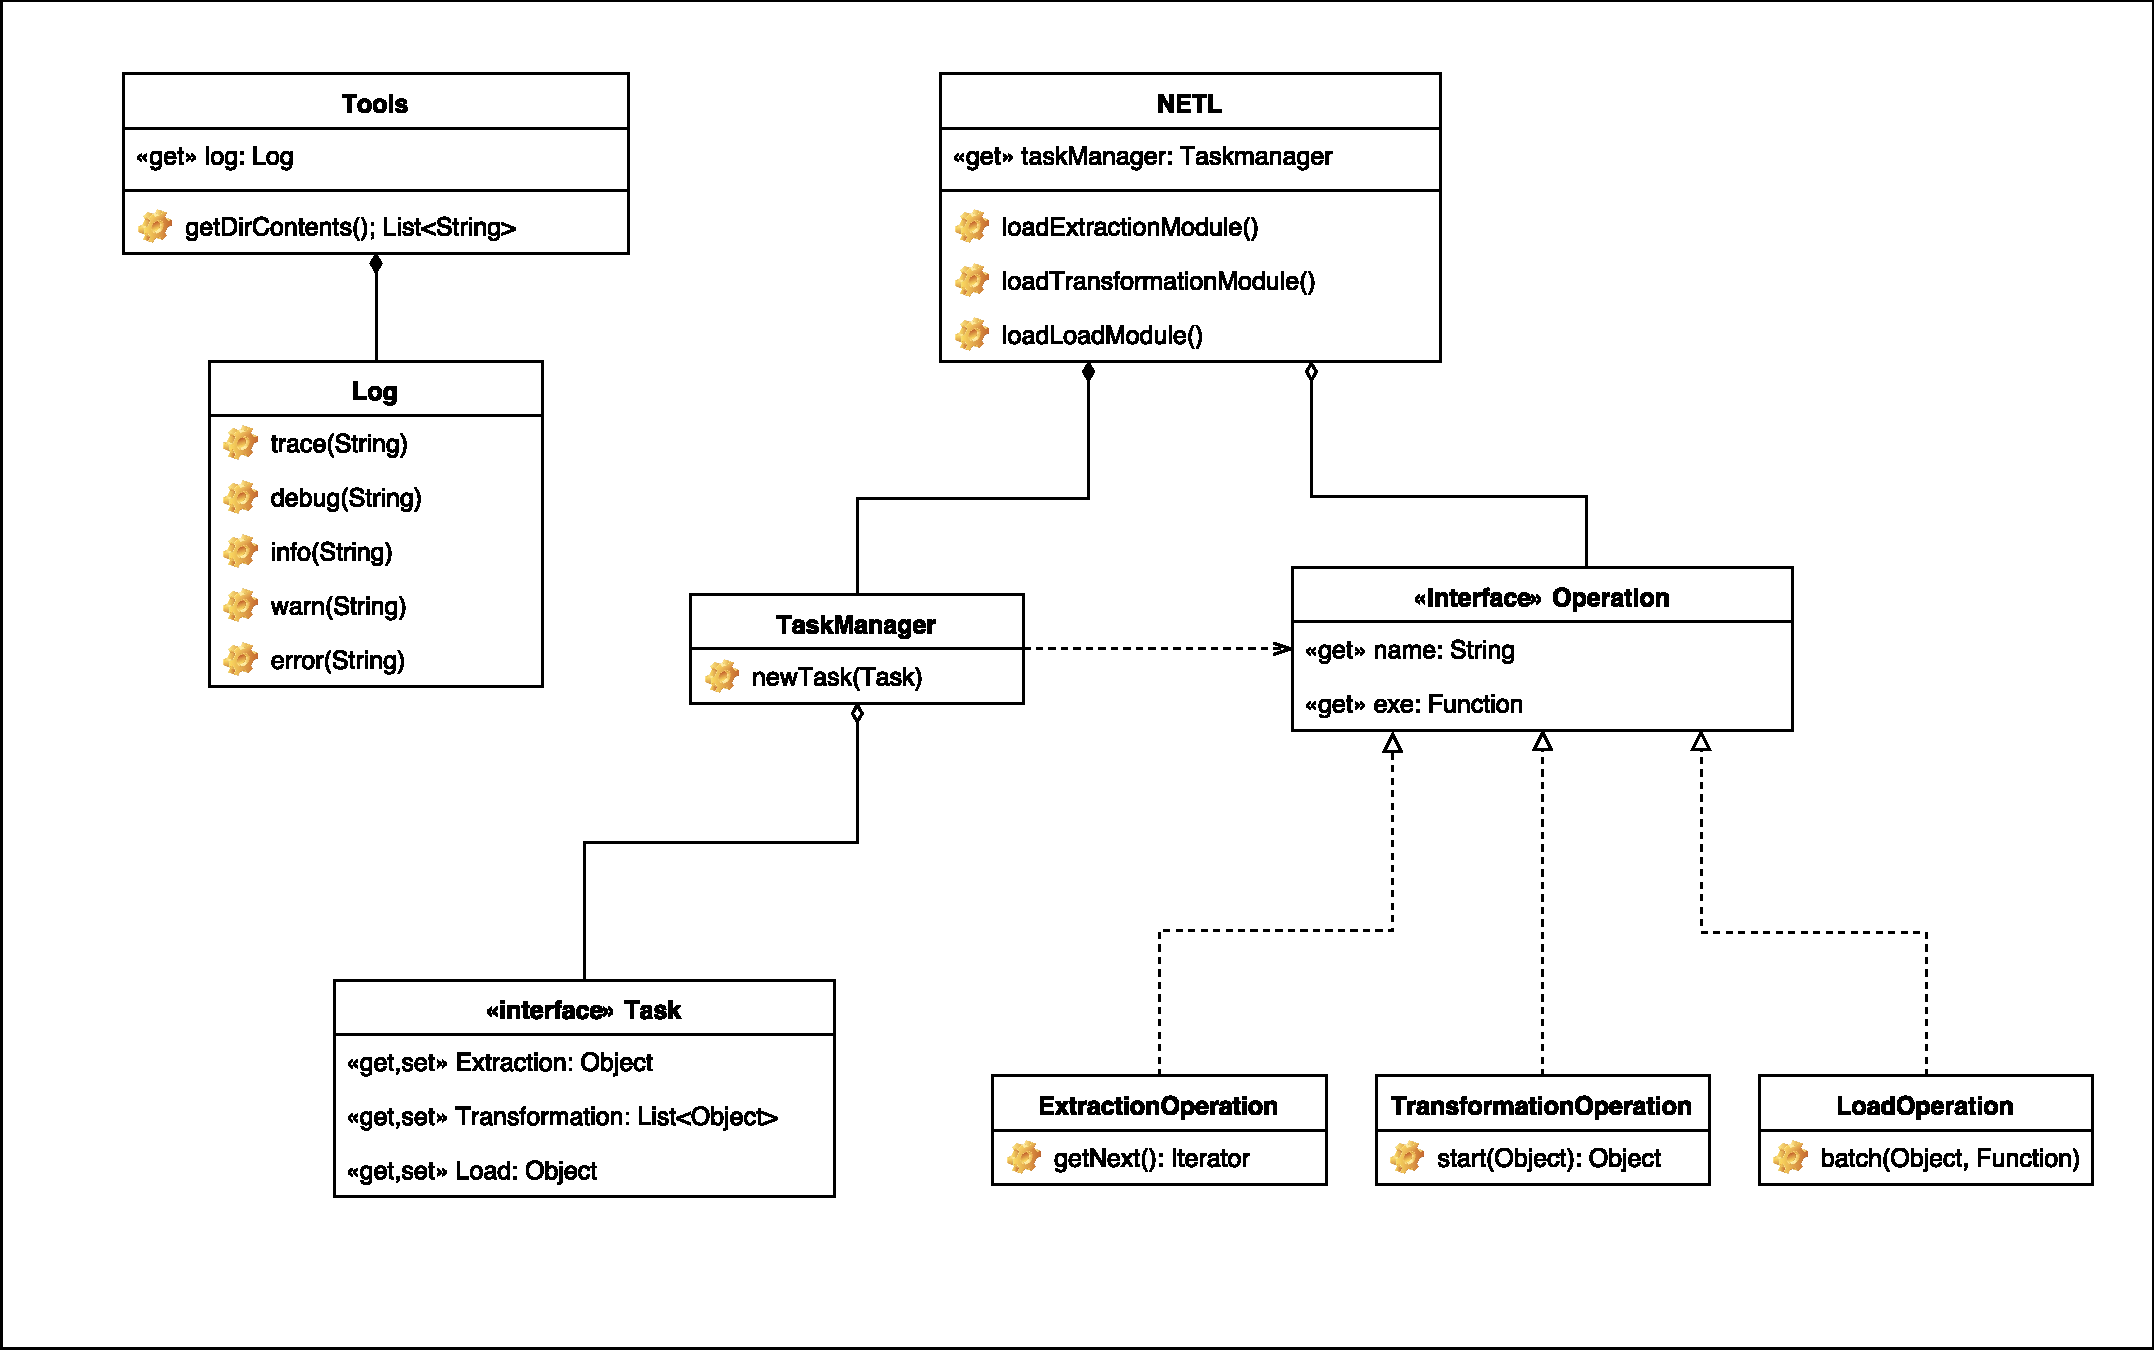
\includegraphics[scale=0.4]{./resources/figures/netlUML}
    \caption[nETL]{nETL}
    \label{nETL}
\end{figure}

Figure \ref{nETL} shows a potential architecture for a configurable component-based ETL tool. The intention of the framework is that it works on the basis of a pipeline of tasks. These tasks can be divided into 3 steps; an extraction step, a transformation step and a loading step. xxx insert something about ETL variations and why I chose the ETL pipeline.

\begin{enumerate}
    \item Extract data from a source specified by a user into memory
    \item Apply any number of transformations to the data in memory
    \item Load the data from memory into a destination specified by a user
\end{enumerate}

The framework itself is quite lightweight and comprises just the NETL, TaskManager and general purpose 'Tools' classes. For the purposes of this thesis, the framework as described by Figure \ref{nETL} has been prototyped in node.js with the source code available at xxx (there is also an npm package available at xxx). JavaScript is a suitable language to prototype this application for a number of reasons:

\begin{enumerate}
    \item It has a very succinct API making it fast to write code in (i.e. it is a highly abstracted language similarly to Ruby or Python)
    \item But unlike Ruby or Python (and other high level languages), it is opinionated in that it handles IO asynchronously by default
    \item The JavaScript implementation of object-orientation allows for easy runtime manipulation of the object model
    \item Another reason for choosing JavaScript is that it is very much in line with the spirit of CouchDB and the web in general
\end{enumerate}

nETL is primarily a task-managing application, and as such, the TaskManager class is effectively the core of the application. It is intended that it can be instantiated as an instance (i.e. there can be many TaskManager instances hosted within a single running application). In JavaScript this is best implemented via a constructor:

\begin{minted}{javascript}
/* File taskmanager.js */
function TaskManager(extractions, transformations, loads) {
    this.tasks = {};

    // Hold references to extractions/transformation/loads of the main application process
    this.extractions = extractions;
    this.transformations = transformations;
    this.loads = loads;
};

TaskManager.prototype.newTask = function(task) {
    // Add task to this.tasks and execute the task
};

module.exports = TaskManager;
\end{minted}

The application itself is intended to be singleton instance of \mintinline{javascript}{class NETL{}}, which provides an IO interface (either a console terminal or otherwise) to TaskManager instances, and modular extraction/transformation and load operations. Singleton's are typically implemented via the modular pattern in JavaScript, which is typically how libraries are delivered to users by package managers and invoked by \mintinline{javascript}{var library = require('library-name')();}. One possible way of implementing the NETL class in JavaScript (i.e the method that is used within this project's code base) is shown here:

\begin{minted}{javascript}
/* File netl.js */
module.exports = function() {
    // Private properties / methods
    const _extractions = {};
    const _transformations = {};
    const _loads = {};        
    const _taskManager = new TaskManager(_extractions, _transformations, _loads);
    function _loadExtractionModule(extractionOperation){};
    function _loadTransformationModule(transformOperation){};
    function _loadLoadModule(loadOperation){};

    // Make process API available
    return {
        taskManager: _taskManager,
        loadExtractionModule: _loadExtractionModule,
        loadTransformationModule: _loadTransformationModule,
        loadLoadModule: _loadLoadModule
    };
};
\end{minted}
\subsubsection{Implementation}
Since extraction \ensuremath{\rightarrow} transformation \ensuremath{\rightarrow} load pipelines are defined via user-configuration, line data-structures can effectively be replaced by any data structure a user desires. Of course that user needs to make sure that the pipeline component (module) at any point in the pipeline can handle the data structure passed to it.

In any case, once a batch of x lines (or any other kind of data structure) has been obtained, transforming and loading data is pretty easy. Pseudocode to implement the nETL framework task-engine could be written something along the lines of:

\begin{minted}{javascript}
// An IIFE is used effectively as an asynchronous implementation of a while loop
(function doEtlTask(self) {
    var payLoad = [];
    var batch = getBatch.next();

    // Apply transformations to elements of extracted batch
    batch.forEach(function(datum){
        SpecifiedTransformations.forEach(function(t) {
            datum = self.transformations[t.Name].call(t, t).start(datum);
        });
        payLoad.push(datum);
    });

    // Load the batch
    self.load.batch(payLoad, function(status, msg) {
        doEtlTask(self); // Start ETL of next batch
    });

})(/* bind task configuration object to function execution context */);
\end{minted}

\subsection{Usage}
Packaged as a node.js module, the intention is that a user can simply import the \mintinline{javascript}{NETL} module and instantiate the \mintinline{javascript}{NETL} class as a singleton. Thereafter a user can add their own extraction / transformation / load modules via the singleton's API (the returned object). The format of these modules should conform to the interface as represented in the diagram. (Actually, JavaScript is not a suitable language for specifying interfaces since tooling that allows interface implementation in the language easy is lacking).

As specified in Figure \ref{nETL}, modules should return an object with the properties 'name' and 'exe'. 'name' should be the naming identifier of the function, and 'exe' should return the starting function of the module. Adding modules to the framework makes them available to tasks as specified by configuration objects. These objects are implemented as a JSON, and are used as instructions to start Tasks. Effectively this allows users to specify custom data processing tasks as a configuration + module. The configuration is passed to the program on startup, and the tasks are run. A possible netl startup script with in line configuration and modules may look like this:

\begin{minted}{javascript}
/* File <user entry point>.js */

// Import the nETL module
const NETL = require('./path/to/netl.js');
var netl = NETL();

// Specify the extraction/transformation/load configuration
const config = [{
    "ID": "TaskName",
    "Extraction": {
        "Name": "ExtractionType",
        // ...
        "afterTaskRunCBs": ["function(moduleConfig) {console.log('Run on task-end')}"]
    },
    "Transformations": [{
            "Name": "TransType",
            // ...
            "afterTaskRunCBs": ["function(moduleConfig) {console.log('Run on task-end')}"]
        },
        {
            // ...
        },
        // ...
    ],
    "Load": {
        "Name": "LoadType",
        // ...
        "afterTaskRunCBs": ["function(moduleConfig) {console.log('Run on task-end')}"]
    }
}];

// Load your own bespoke extraction module
netl.loadExtractionModule((function() {
    function exe(obj) {
        // ...
    };
    return {
        name: "ExtractionType",
        exe: exe
    };
})());

// Load your own bespoke Transformation module
netl.loadTransformationModule((function() {
    function exe(obj) {
        // ...
    };
    return {
        name: "TransType",
        exe: exe
    };
})());

// Load your own bespoke Load module
netl.loadLoadModule((function() {
    function exe(obj) {
        // ...
    };
    return {
        name: "LoadType",
        exe: exe
    };
})());

// Run your task till completion
netl.taskManager.newTask(config);
\end{minted}
\subsubsection{Extractions}
The framework above has been conceptualized primarily as a means of working with CSV data as exported from the Sukai platform. Specifically, this MSc has the dual requirements of extracting data from an 80GB CSV and snonymising column(s) in this 80GB CSV in a predictable way. To this end, included in the nETL source code used to complete this thesis is a FLATFILE extraction module.

Ethical clearance to use student data, although granted by the University of Cape Town still makes the condition that identities of the students be anonymized. Partly as a way of testing the nETL framework as mentioned above, I offered to provide a 'one-click' installation of the nETL application that provides an anonymizing pipeline for use by Professor Sonia Berman to prepare the student data for this project.

Extracting data from a flatfile is only tricky if it's size is such that the memory footprint of file contents is greater than the memory made available to the process. For an 80GB CSV that is certainly the case. The only feasible means of extracting data from such a file is to utilize the concept of an 'iterator'. Effectively this involves specifying the size of a reading block via two pointers (a 'begin' and 'end' pointer) that then traverse the data structure of the file from start to finish. These pointers maintain a constant width apart and at each incrementation of the iteration retrieve the data between those pointers.

Using an iterator, it is straightforward to process portions of a file at time, so long as only partial retrieval of a file's data can still be understood. Flatfile's work well for this with data structured as any number of 'line' entities that don't need to be read in the context of other marker's that may be found within the file.

Almost all high-level languages provide numerous abstractions for reading flatfile's on a line-by-line basis. For example, in a few different languages file iterators can be generated in the following ways:

\paragraph*{Python}
\begin{minted}{python}
with open('/path/to/file') as file:
   for line in file:
       # Process the line
\end{minted}

\paragraph*{Ruby}
\begin{minted}{ruby}
IO.foreach('/path/to/file') do |line|
  # Process the line
end
\end{minted}

\paragraph*{C\#}
\begin{minted}{csharp}
using (StreamReader streamReader = File.OpenText(/path/to/file))
{
    string line = String.Empty;
    while ((line = streamReader.ReadLine()) != null)
    {
        // Process the line
    }
}
\end{minted}

JavaScript provides a similar API for reading files line-by-line to the languages mentioned above, and a user could write such a simple iterator module provided that the module adhere to the nETL module interface for extractions and implements a \mintinline{javascript}{getNext()} function that effectively allows for pausing such extraction. It's likely that there are numerous ways of achieving this with the standard ECMAScript 5 standard. But partly as a means of exploring more state-of-the art JavaScript features, and partly of a means of demonstrating these new features, the file extraction module as used in this thesis implements EcmaScript 6 generators.

As described by \cite{mozillaGenerators}, JavaScript generators allow for quickly implementing arbitrary iterators, including iterators over generated iterators. Using open source code provided by \cite{bower16}, nETL makes use of a generator function to create a file iterator, and then a higher level generator to iterate over results of the line generator:

\begin{minted}{javascript}
var pointer = 0;
var buffersize = 64KB; // As close to a disc read size as possible
var filesize = FileLength;

// Generate the filereader
function* _readLines() {
    while (pointer < filesize) {
        let lineBuffer = [];
        // 1. Create a dataBuffer (byte array) of the data between pointer and filesize
        // 2. Find the start of a line
        // 3. Iterator through dataBuffer until a newline marker is found
            // Load each byte into lineBuffer
        // 4. yield lineBuffer.toString
    };
};
var lineReader = _readLines();

// Simplified implimentation of getNext() public API
function getNext() {
    return lineReader.next();
};

// Simplified batch generator
function getBatch* () {
    let data = [];
    for (0..batchSize) {
        data.push(lineExtraction.getNext());
    };
    yield data;
};

// Then batches of lines can be extracted via the following code
var batch = getBatch.next();
\end{minted}

compared to implementing an iterating-linereader in other languages, the JavaScript syntax in this case is more verbose. However this is largely because of the opinionated, asynchronous approach to IO operations. This approach makes the nETL framework easier to implement as a whole, however, since it allows many JavaScript tasks to run asynchronously. This would be harder to implement in languages such as Ruby/Python/C\#/etc and would probably involve some kind of thread management. This is not required with JavaScript.
\subsubsection{Transformation}
\subsubsection{Load}

\newpage

% Appendix
\begin{appendix}
    \listoffigures
    \listoftables
\end{appendix}
\newpage

% Bibliogrpahy
\bibliographystyle{plain}
\bibliography{bibliography/msc_citations}

% Close docuemnt
\end{document}